\newcommand{\Ps}{\mathcal P}

Using COSY Infinity we compute the Taylor expansion of spin tune $\nu_s(\vec z)$, where
\begin{align*}
  \vec z &= (x,a,y,b,\ell,\delta), \\
  \ell &= -(t - t_0)v_0\frac{\gamma-1}{\gamma}, \\
  \delta &= \frac{\Delta K}{K}.
\end{align*}

In the present section we will test formulation B of Statement 1:
the multivariate function $\nu_s(\vec z)$ can be expressed as a function of a single scalar parameter:
$\nu_s(\g*)$. We will not assume any formal expression of $\g*$.

If formulation B is correct, there exists a coordinate system (with one axis being $\nu_s$),
in which horizontal plane betatron oscillating particles are indistinguishable, in terms of spin tune,
from vertical plane betatron oscillating particles. This coordinate system, hence, must not include
coordinates from the transverse phase space planes $(x,a)$, and $(y,b)$.

Therefore, we will look at the space $\Ps=(\ell, \delta, \nu_s)$. If formulation B is correct,
differences between particles' transverse phase plane trajectories must not reflect on their
trajetctories in $\Ps$.

We used the same data in this analysis as in the previous section.

In Figure~\ref{fig:main:all_ps} $\nu_s(\vec z)$ is plotted as a function of $(\ell, \delta)$ when
$\vec z$ is the real trajectory the particle takes in the storage ring. We observe:
\begin{enumerate}
\item the same stratification of the mean spin tune levels as in figures 
	in section~\ref{sec:decoh:sim-imperfect};
\item the stratification is more pronounced for the X-bunch (blue dots), than for the Y-bunch (red dots).
\end{enumerate}

The latter can be explained by the greater magnitude of the dispersion function in the horizontal plane.
Note that at equal values of the Q-normalized transverse emittance~\footnote{Q-normalized is $\epsilon_\alpha\cdot Q_\alpha$, where $\alpha\in\{x,y\}$.} (i.e. at equal orbit lengthenings, if equation~\eqref{eq:betatron_OL}
is to be believed), horizontal plane betatron oscillating particles have a greater longitudinal emittance than
those oscillating in the vertical plane.

\begin{figure}[h]
  \centering
  \begin{subfigure}{\linewidth}
    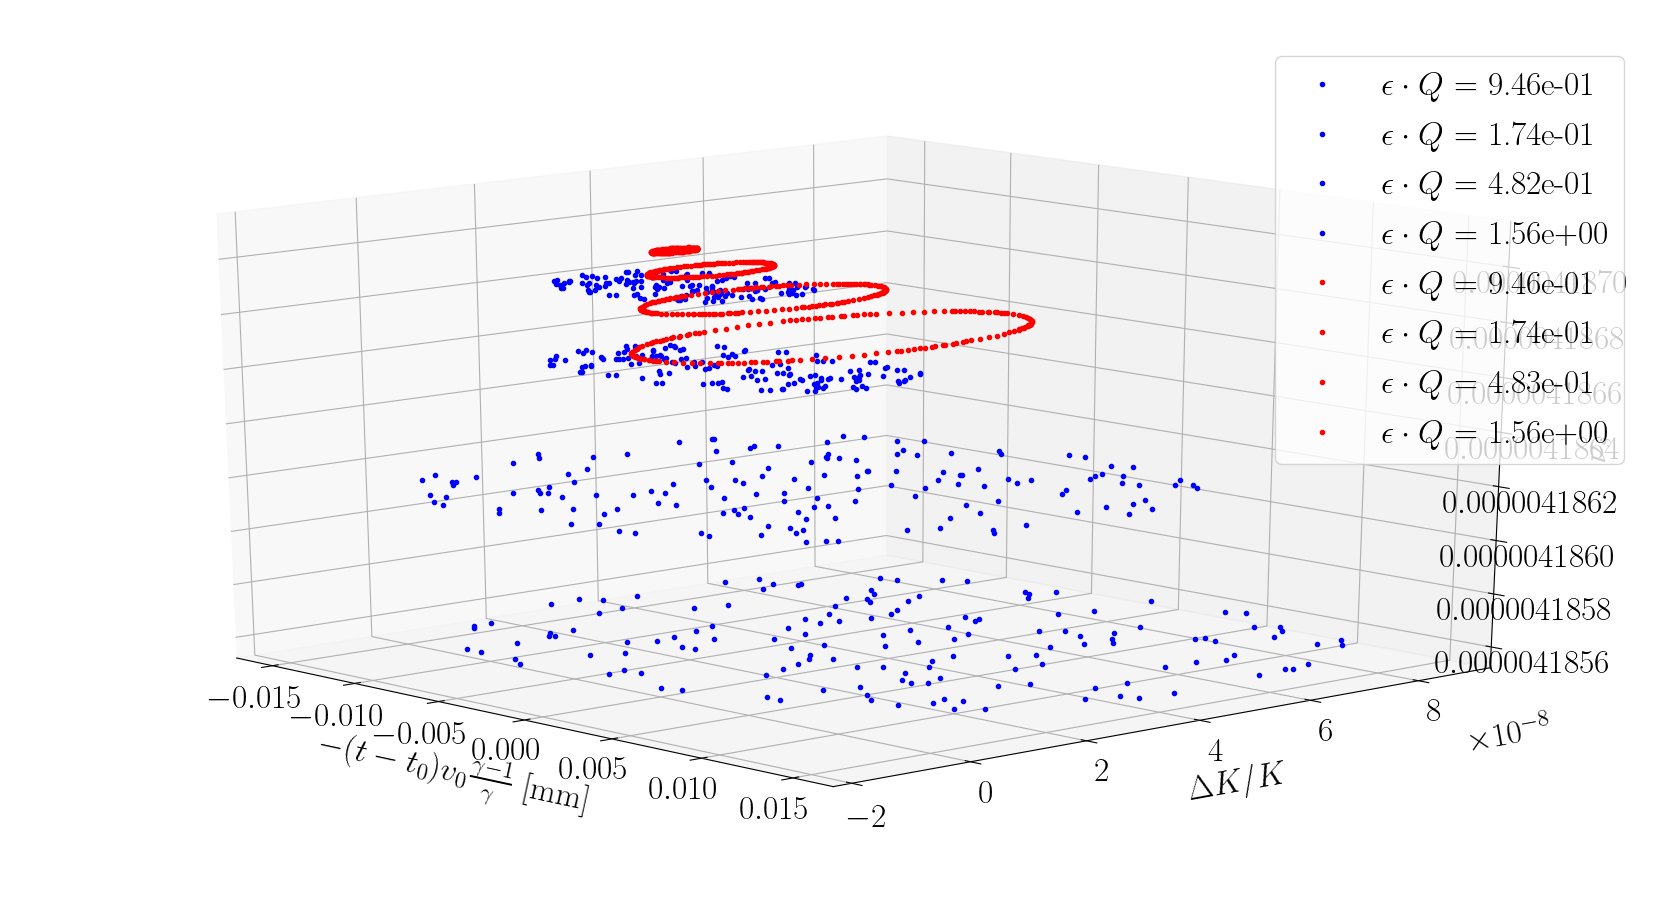
\includegraphics[height=.3\paperheight]{images/stune_traj_equ/part2/3D_plot_all_ps_vars}
    \caption{Particles picked according to the values of their Q-normalized \emph{transverse}
    emittances.\label{fig:main:all_ps}}
  \end{subfigure}
  \begin{subfigure}{\linewidth}
    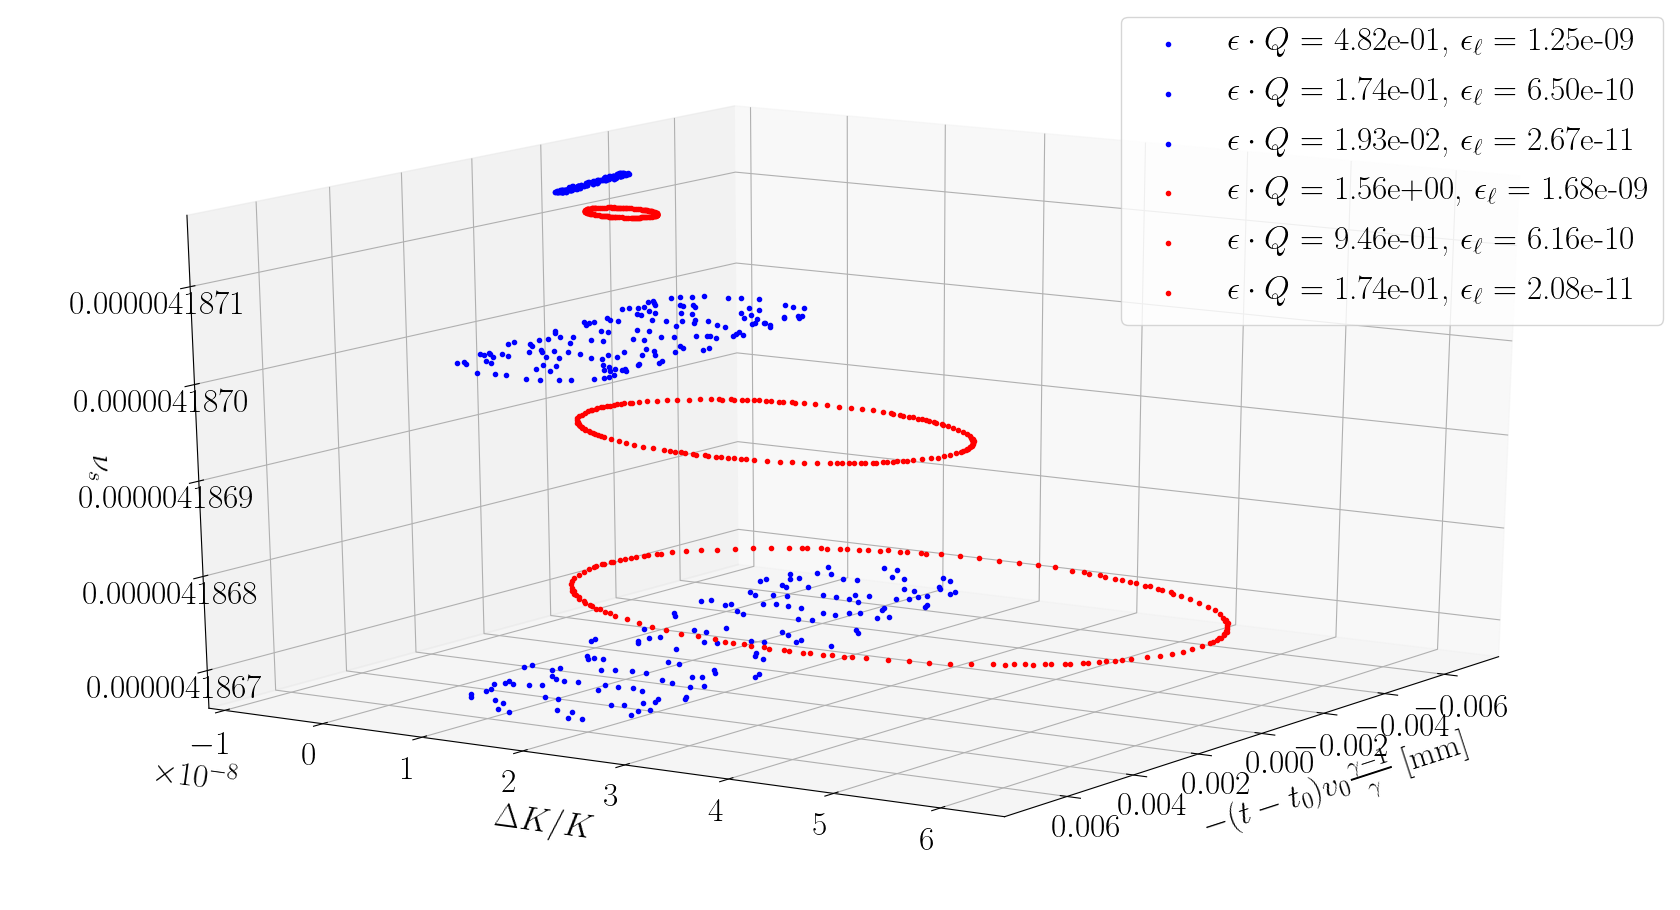
\includegraphics[height=.3\paperheight]{images/stune_traj_equ/part2/3D_plot_all_ps_vars_equal_long_emi}
    \caption{Particles are picked according to the values of their \emph{longitudinal}
    emittances.\label{fig:main:gamma_eff}}
  \end{subfigure}
  \caption{Spin tune as a function of the particle's position in the longitudinal phase space.
    Colors mark the bunch: blue for X, red for Y. The corresponding Q-normalized transverse and
    longitudinal emittances are shown in the legend.\label{fig:main}}
\end{figure}

Due to this fact, we decided to plot the same dependence, but to pick particles based on the equality of
their longitudinal, instead of transverse, emittances. In Figure~\ref{fig:main:gamma_eff} we observe that
particles having similar magnitudes of their longitudinal emittance have also silimar mean spin tune levels.

\paragraph{Conclusion:} formulation B is confirmed by simulation; the effective Lorentz factor reflects the
magnitude of the particle's longitudinal emittance.

In view of Figure~\ref{decoh:fig:nbar_vs_ST}, one can also conclude that particles with equal
effective L-factor values are spin dynamics-equivalent in the general sense, by which we mean that
they have not only equal values of spin tune, but the same orientation of the invariant spin axis.~\footnote{
At any rate, this seems to be true in the FS regime of operation.}
